% ============================================================
%  Informe tecnico — EL-5409 Laboratorio de Control Automatico
%  Proyecto final: Model-Based Design para la planta Ball on Plate
%  Formato IEEE, dos columnas. Compilar con pdfLaTeX + BibTeX
%  (latexmk -pdf informe.tex).
%
%  PLANTILLA: los recuadros rojos (\pendiente y \figpendiente)
%  marcan lo que falta. Antes de entregar, cambiar a
%  \mostrarpendientesfalse en preambulo.tex y revisar que no
%  quede ninguno.
%
%  Todos los numeros salen de archivos del repo (ver LEEME.md de
%  esta carpeta). No se escriben valores que no tengan respaldo.
% ============================================================
\documentclass[conference,a4paper,10pt]{IEEEtran}

% ============================================================
%  Preambulo — Informe IEEE (dos columnas) · Proyecto final EL-5409 (Ball on Plate)
% ============================================================

\usepackage[T1]{fontenc}
\usepackage[utf8]{inputenc}
\usepackage[spanish,es-tabla,es-noquoting]{babel}
\usepackage{amsmath,amssymb}
\usepackage{graphicx}
\usepackage{booktabs}
\usepackage{array}
\usepackage{enumitem}
\usepackage{listings}
\usepackage{xcolor}
\usepackage{balance}
\usepackage{xurl}          % permite cortar URLs largas en la bibliografia
\usepackage[hidelinks,unicode]{hyperref}

% IEEEtran define \IEEEproof etc.; evitamos choques de babel
\addto\captionsspanish{\renewcommand{\tablename}{TABLA}}

% ---------- Unidades ----------
\usepackage{siunitx}
\sisetup{
  output-decimal-marker = {,},
  group-separator       = {\,},
  per-mode              = symbol,
  detect-all            = true
}

% ---------- Graficas ----------
\usepackage{pgfplots}
\usepackage{pgfplotstable}
\pgfplotsset{compat=1.18}
\usepgfplotslibrary{groupplots}
\usetikzlibrary{matrix,positioning,fit}

% Ruta a la carpeta de datos
\newcommand{\G}{datos_graficas}

\definecolor{cAzul}   {HTML}{1F4E79}
\definecolor{cNaranja}{HTML}{C55A11}
\definecolor{cVerde}  {HTML}{2E7D32}
\definecolor{cGris}   {HTML}{6E6E6E}
\definecolor{cRojo}   {HTML}{A61C1C}

% Estilo base: pensado para una columna IEEE
\pgfplotsset{
  estilo/.style={
    width            = 0.97\columnwidth,
    height           = 4.1cm,
    scale only axis  = false,
    grid             = major,
    grid style       = {gray!20, line width=0.25pt},
    tick label style = {font=\scriptsize},
    label style      = {font=\scriptsize},
    legend style     = {font=\scriptsize, draw=gray!45, fill=white,
                        fill opacity=0.85, text opacity=1,
                        inner sep=1.5pt, row sep=-1pt},
    legend cell align = left,
    every axis plot/.append style = {line width=0.7pt},
    scaled ticks = false,
    tick align   = outside,
    max space between ticks = 40pt,
  },
  ancho/.style = {width=0.47\textwidth, height=4.3cm},
  aligera/.style = {each nth point=#1, filter discard warning=false,
                    unbounded coords=discard},
  aligera/.default = 4,
}

% ---------- Codigo fuente ----------
\lstdefinestyle{estiloC}{
  language=C, basicstyle=\ttfamily\scriptsize,
  keywordstyle=\color{cAzul}\bfseries,
  commentstyle=\color{cGris}\itshape,
  frame=single, rulecolor=\color{gray!40},
  breaklines=true, showstringspaces=false, columns=fullflexible,
  xleftmargin=0.6em, aboveskip=4pt, belowskip=2pt
}
\lstset{style=estiloC}

% ---------- Marcas de trabajo pendiente ----------
% Cambie a \mostrarpendientesfalse antes de entregar
\newif\ifmostrarpendientes
\mostrarpendientesfalse
\newcommand{\pendiente}[1]{%
  \ifmostrarpendientes
    \par\noindent\fcolorbox{cRojo}{red!4}{%
      \parbox{0.95\columnwidth}{\scriptsize\color{cRojo}\textbf{PENDIENTE:} #1}}\par\smallskip
  \fi}

% ---------- Figura pendiente (marco vacio con la descripcion) ----------
\newcommand{\figpendiente}[2][3.2cm]{%
  \fbox{\parbox[c][#1][c]{0.92\columnwidth}{\centering\scriptsize\color{cRojo}%
  \textbf{FIGURA PENDIENTE}\\[2pt]#2}}}

% ---------- Atajos ----------
\newcommand{\xh}{\hat{x}}
\newcommand{\vh}{\hat{v}}
\newcommand{\thc}{\theta_{\mathrm{cmd}}}
\newcommand{\thlim}{\theta_{\mathrm{lim}}}
\newcommand{\Xm}{X_m}
\newcommand{\hef}{h_{\mathrm{ef}}}
\newcommand{\hsup}{h_{\mathrm{sup}}}
\newcommand{\Kp}{K_p}
\newcommand{\Kd}{K_d}
\newcommand{\Ki}{K_i}
\newcommand{\Ti}{T_i}
\newcommand{\Ts}{T_s}


\begin{document}

\title{Diseño basado en modelos de un controlador de posición\\
para una planta \emph{Ball on Plate} de dos grados de libertad}

\author{%
\IEEEauthorblockN{Abner López Méndez, 2022273075 \qquad Jordi Segura Chinchilla, 2022240646\\
Anthony Villalta, \textit{carné} \qquad Yonaikel Tencio, \textit{carné}}
\IEEEauthorblockA{Escuela de Ingeniería Electrónica, Tecnológico de Costa Rica\\
EL-5409 --- Laboratorio de Control Automático, II Semestre 2026\\
Profesor: Ing. Juan Luis Guerrero Fernández, PhD}}

\maketitle

\begin{abstract}
\pendiente{Escribir el resumen al final, cuando estén cerradas la identificación (Etapa B), el
rediseño y la implementación física (Etapa H). Debe incluir resultados cuantitativos de cada
etapa. Nombres completos y carnés de Anthony y Yonaikel en el encabezado.}
Se documenta el desarrollo de un controlador de posición para una planta \emph{Ball on Plate}
de dos grados de libertad, en la que una bola rueda sobre un plato que inclinan dos servos y una
cámara cenital mide su posición. Siguiendo un flujo de diseño basado en modelos, se obtuvo un
modelo no lineal por el método de Lagrange y su linealización, un doble integrador por eje,
que no es estable en lazo abierto. Se diseñó un controlador PD por asignación de polos con
integración condicional, que en simulación \emph{Model-in-the-Loop} cumple los requisitos con un
tiempo de establecimiento de \SI{1.30}{\second} y un sobreimpulso de \SI{4.4}{\percent}. El
código generado con Embedded Coder reprodujo exactamente el modelo en
\emph{Software-in-the-Loop} y en \emph{Processor-in-the-Loop} sobre una ESP32, con igualdad en
\num{271} de \num{271} muestras. La identificación en lazo cerrado sobre el prototipo dio una
ganancia efectiva de rodadura cercana a \num{0.2}, frente a \num{0.714} del modelo, y un retardo
de unos \SI{0.3}{\second}.
\end{abstract}

\begin{IEEEkeywords}
Ball on plate, diseño basado en modelos, doble integrador, identificación en lazo cerrado,
integración condicional, SIL, PIL, ESP32, Embedded Coder.
\end{IEEEkeywords}

\section{Introducción}

La planta \emph{Ball on Plate} es una bola que rueda sobre un plato cuadrado de acrílico de
\SI{300}{\milli\metre} $\times$ \SI{300}{\milli\metre}. El plato se apoya en una junta universal central y se inclina en
dos ejes, $\theta_x$ y $\theta_y$, con dos servos Tower Pro MG90D que lo empujan mediante
varillas. Una cámara web cenital, a \SI{450}{\milli\metre} sobre el plato, mide la posición de
la bola. La visión corre en una PC con Linux: segmenta la bola por color, convierte píxeles a
milímetros con una homografía y estima la posición y la velocidad con un filtro de Kalman. El
controlador corre en una ESP32, que recibe el estado por el puerto serie y genera el PWM de los
servos. La variable controlada es la posición $(x, y)$ del centro de la bola, en milímetros, y
la variable manipulada es la inclinación del plato, en grados.

El problema de control consiste en llevar la bola a una posición de referencia y mantenerla ahí
sin que salga del área útil del plato, $|x|, |y| \le \SI{127}{\milli\metre}$, con una inclinación
limitada por el recorrido de los servos. A diferencia de una planta térmica, esta no tiene un
equilibrio estable: sin control, cualquier inclinación lleva la bola al borde en alrededor de un
segundo. Además, el periodo de muestreo no es libre, porque lo fija la cámara a
\SI{30}{fps}, y la cadena de medición agrega un retardo que es tiempo muerto dentro del lazo.

El enunciado del proyecto pide aplicar el flujo de diseño basado en modelos con dos
estrategias de control distintas, validar ambas hasta la simulación \emph{Model-in-the-Loop} y
llevar una de ellas hasta la implementación física. No fija requisitos numéricos, así que los de
la Tabla~\ref{tab:requisitos} los fijó el equipo como una decisión de ingeniería.

\begin{table}[!t]
\caption{Requisitos de desempeño fijados por el equipo. Ensayo: bola quieta a
\SI{100}{\milli\metre} del centro en un eje y referencia en 0.}
\label{tab:requisitos}
\centering
\footnotesize
\setlength{\tabcolsep}{4pt}
\begin{tabular}{@{}lll@{}}
\toprule
\textbf{Id} & \textbf{Requisito} & \textbf{Criterio} \\
\midrule
R1 & Tiempo de establecimiento & $t_s \le \SI{3}{\second}$ (banda del \SI{5}{\percent}) \\
R2 & Sobreimpulso & $M_p \le \SI{20}{\percent}$ \\
R3 & Error estacionario & $e_{ss} \le \SI{3}{\milli\metre}$ \\
R4 & Seguridad & $|x|, |y| \le \SI{127}{\milli\metre}$ siempre \\
Diseño & Márgenes del lazo lineal & $\mathrm{PM} \ge \SI{40}{\degree}$, $\mathrm{GM} \ge \SI{6}{\deci\bel}$ \\
\bottomrule
\end{tabular}
\end{table}

Las métricas se calculan siempre sobre la posición filtrada $\xh$ en los instantes de cuadro,
que es lo que registra la PC, para que la misma definición sirva en simulación y en el
experimento: $t_s$ es el último instante con $|\xh - r|$ mayor que el \SI{5}{\percent} del
cambio, $M_p$ el máximo sobrepaso en porcentaje del cambio y $e_{ss}$ el valor absoluto de la
media del error en el último segundo.

Como en el Proyecto~1, el objetivo no es solo que el controlador funcione en simulación, sino
recorrer el flujo completo de diseño basado en modelos \cite{mw_hil}:

\begin{center}
modelado $\rightarrow$ identificación $\rightarrow$ diseño $\rightarrow$ MIL $\rightarrow$
código $\rightarrow$ SIL $\rightarrow$ PIL $\rightarrow$ implementación física.
\end{center}

El orden real del trabajo no fue estrictamente ese. Para avanzar mientras se terminaba el
prototipo, el diseño, el MIL, la generación de código, el SIL y el PIL se hicieron primero con el
modelo físico, y la identificación con el prototipo se hizo después. Por eso la
Sección~II presenta el modelo identificado, pero los controladores de la Sección~III se
diseñaron con el modelo físico; la Sección~VII analiza esa diferencia. Las dos estrategias fueron
un PID con integración condicional y un LQR con acción integral; el PID es el que continuó hasta
la implementación.

\section{Modelado e identificación del sistema}

\subsection{Modelo físico}

El modelo se planteó desde primeros principios, con las ecuaciones de Lagrange para la bola
sobre el plato. Las hipótesis fueron: la bola rueda sin deslizar y no gira alrededor de la normal
del plato; es rígida, con momento de inercia $J = k\,m\,r_b^2$; el plato y el mecanismo son
rígidos y sin holgura; no hay fricción de rodadura; la entrada del modelo es la inclinación del
plato, con el actuador modelado aparte; y la cámara está fija sobre el eje de la junta. Se define
el coeficiente de rodadura $c = 1/(1+k)$, que vale $5/7$ para una esfera maciza. La masa de la
bola se cancela.

Para un eje, con el otro horizontal, la ecuación queda

\begin{equation}
\ddot x = c\left[-g\sin\theta + x\,\dot\theta^{2} + \hef\,\ddot\theta\right],
\qquad \hef = h + k\,r_b,
\label{eq:nolineal}
\end{equation}

donde $h$ es la altura del centro de la bola sobre el centro de la junta. El modelo completo de
dos ejes agrega términos de Coriolis y de acople que solo aparecen cuando los dos ejes se mueven
a la vez. Las no linealidades son el seno, el término centrífugo $x\,\dot\theta^{2}$, la
proyección que hace la cámara cuando el plato está inclinado, el mecanismo de cuatro barras
entre servo y plato, y la saturación y la velocidad máxima del servo.

La cámara no mide la posición sobre el plato. Como la homografía se calibró con el plato
horizontal, con el plato inclinado mide la proyección del centro de la bola, que linealizada da
$\Xm = x - h\,\theta$. Linealizando \eqref{eq:nolineal} alrededor de $x = \dot x = 0$,
$\theta = \dot\theta = 0$, se obtienen dos funciones de transferencia por eje,

\begin{align}
\frac{X(s)}{\Theta(s)} &= \frac{c\,\hef\,s^{2} - c\,g}{s^{2}},
\label{eq:lineal}\\
\frac{\Xm(s)}{\Theta(s)} &= \frac{-(1-c)\,\hsup\,s^{2} - c\,g}{s^{2}},
\label{eq:linealm}
\end{align}

donde $\hsup$ es la altura de la cara del plato sobre la junta. El jacobiano del modelo de dos
ejes en el punto de operación no tiene términos cruzados (diferencia relativa con el analítico de
\num{1.7e-13}), así que a primer orden los ejes quedan desacoplados y se tratan como dos lazos
SISO iguales. La Tabla~\ref{tab:fisico} resume los valores con la geometría del diseño.

\begin{table}[!t]
\caption{Modelo lineal por eje con los parámetros del diseño ($c = 5/7$,
$\hsup = \SI{49}{\milli\metre}$, $h = \SI{69}{\milli\metre}$, $r_b = \SI{20}{\milli\metre}$).
Fuente: \texttt{etapaA/resultados/A2\_consola.txt}.}
\label{tab:fisico}
\centering
\footnotesize
\begin{tabular}{@{}lr@{}}
\toprule
\textbf{Magnitud} & \textbf{Valor} \\
\midrule
$c\,g$ & \SI{7007}{\milli\metre\per\second\squared\per\radian} \\
$c\,\hef$ & \SI{55.0}{\milli\metre\per\radian} \\
$-(1-c)\,\hsup$ & \SI{-14.0}{\milli\metre\per\radian} \\
Polos & $s = 0$ (doble) \\
Ceros de $X/\Theta$ & $s = \pm\SI{11.29}{\radian\per\second}$ \\
Ceros de $\Xm/\Theta$ & $s = \pm j\,\SI{22.37}{\radian\per\second}$ \\
Pendiente servo $\rightarrow$ plato (diseño) & \SI{0.343}{\degree\per\degree} \\
\bottomrule
\end{tabular}
\end{table}

El doble polo en el origen tiene tres consecuencias que salen del modelo. Primero, la planta no
es estable en lazo abierto: con \SI{2}{\degree} de inclinación la bola llega a la pared en
aproximadamente \SI{1.0}{\second}, de modo que un ensayo escalón en lazo abierto no es posible.
Segundo, el método SIMC usado en el Proyecto~1 no aplica, porque supone una planta estable de
primer orden con tiempo muerto \cite{skogestad2003}. Tercero, un PI no puede estabilizar un doble
integrador: hace falta acción derivativa o realimentación de velocidad.

Para cuantificar el error de la aproximación lineal no se pueden usar escalones, porque la planta
no tiene equilibrio estable. Se aplicó un triplete de inclinación ($+A$, $-A$, $+A$) que, en el
modelo lineal, deja la bola en reposo en el punto de partida, con transiciones rápidas (el plato
a la velocidad máxima del servo, unos \SI{206}{\degree\per\second}) y lentas. La
Fig.~\ref{fig:barrido} muestra el error de trayectoria en función de la amplitud. Con el criterio
fijado por el equipo, un error menor al \SI{5}{\percent} de $\max|x|$, el modelo lineal vale
hasta $A = \SI{3}{\degree}$ con transiciones lentas, pero solo hasta \SI{0.5}{\degree} con
transiciones rápidas. El término dominante no es el seno, que a \SI{13}{\degree} equivale a solo
\SI{0.11}{\degree} de error de inclinación, sino el centrífugo $x\,\dot\theta^{2}$, que crece con
el cuadrado de la velocidad del plato. Por eso conviene que el controlador no pida cambios
bruscos de inclinación.

\begin{figure}[!t]
\centering
\begin{tikzpicture}
\begin{axis}[estilo, height=3.8cm, xlabel={Amplitud del triplete $A$ (\si{\degree})},
             ylabel={Error de trayectoria (\si{\percent})}, ymin=0, ymax=100, xmin=0, xmax=13.5,
             legend pos=north west]
  \addplot[cRojo, mark=*, mark size=1pt]
    table[col sep=comma, x=A_deg, y=err_rel_x_pct,
          restrict expr to domain={\thisrow{modo_1rapida_2lenta}}{1:1}] {\G/A2_barrido_amplitud.csv};
  \addplot[cAzul, mark=square*, mark size=1pt]
    table[col sep=comma, x=A_deg, y=err_rel_x_pct,
          restrict expr to domain={\thisrow{modo_1rapida_2lenta}}{2:2}] {\G/A2_barrido_amplitud.csv};
  \addplot[cGris, dashed, domain=0:13.5, samples=2] {5};
  \legend{Transición rápida, Transición lenta, Umbral \SI{5}{\percent}}
\end{axis}
\end{tikzpicture}
\caption{Error del modelo lineal frente al no lineal, en porcentaje de $\max|x|$, para el
triplete de inclinación con transiciones rápidas y lentas.}
\label{fig:barrido}
\end{figure}

\subsection{Caracterización del sensor y del actuador}

Antes de identificar la dinámica de la bola se midieron, sobre el prototipo, los elementos de la
cadena que el modelo trataba como ideales. La Tabla~\ref{tab:caracterizacion} resume las
mediciones.

\begin{table}[!t]
\caption{Mediciones de la cadena de medición y del actuador sobre el prototipo. Fuente:
\texttt{datos\_prototipo/camara/} y \texttt{datos\_prototipo/mecanica/}.}
\label{tab:caracterizacion}
\centering
\footnotesize
\begin{tabular}{@{}lr@{}}
\toprule
\textbf{Magnitud} & \textbf{Valor medido} \\
\midrule
Periodo entre cuadros (YUYV, 2 búferes) & \SI{33.25}{\milli\second}, desv. \SI{1.9}{\milli\second} \\
Cuadros dentro de $\pm\SI{5}{\milli\second}$ / perdidos & \SI{100}{\percent} / \SI{0}{\percent} \\
Latencia de la visión (mediana, 2 corridas) & \SI{57.8}{} y \SI{60.3}{\milli\second} \\
Ruido de posición, bola quieta (centro / esquina) & \SI{0.12}{} / \SI{0.09}{\milli\metre} \\
Pendiente servo $\rightarrow$ plato cerca del neutro (v3) & \SI{0.47}{\degree\per\degree} \\
Holgura del mecanismo (eje X / eje Y) & hasta \SI{0.8}{} / \SI{2.4}{\degree} \\
\bottomrule
\end{tabular}
\end{table}

El periodo de muestreo quedó en $\Ts = \SI{33.3}{\milli\second}$ con el formato YUYV y dos
búferes; el MJPG se descartó porque perdía el \SI{46}{\percent} de los cuadros. La latencia
medida, de unos \SI{60}{\milli\second}, quedó por debajo de los \SI{75}{\milli\second} que se
habían estimado para el diseño. La relación entre el ángulo del servo y el del plato resultó
asimétrica y con una pendiente cerca de 1,4 veces la del diseño, así que el firmware convierte
la inclinación pedida en comando del servo con la tabla medida y no con la cinemática del diseño.
Con esa tabla, el peor eje alcanza unos $\pm\SI{11.3}{\degree}$, y la saturación del controlador
se fijó en $\thlim = \SI{10}{\degree}$. La tabla vigente es la v3, medida el 2026-11-09 después
de reajustar los brazos de los servos.

\subsection{Identificación experimental}

Como la planta no es estable en lazo abierto, la identificación se hizo en lazo cerrado. El
firmware de prueba de la ESP32 ejecuta un ensayo automático con escalones de referencia, una
perturbación pseudoaleatoria de $\pm\SI{1.5}{\degree}$ sumada a la inclinación y trayectorias
circulares, y devuelve en cada cuadro la inclinación que aplicó. Con esa telemetría y la posición
medida se ajustó, por mínimos cuadrados y en ventanas de \SI{1}{\second}, el modelo por eje

\begin{equation}
\ddot x = -c_{\mathrm{ef}}\,g\,\sin\theta(t-\tau) + b - f\,\operatorname{sign}(\dot x),
\label{eq:b3}
\end{equation}

donde $c_{\mathrm{ef}}$ es una ganancia de rodadura efectiva, que incluye también la ganancia
real de la transmisión servo--plato, $b$ representa un desnivel constante, $f$ un rozamiento o
zona muerta, y $\tau$ el retardo entre la orden de inclinación y la respuesta de la bola. El
retardo se buscó en una grilla, minimizando el error de ajuste. En la Fig.~\ref{fig:tau}, el
mínimo está en \SI{340}{\milli\second} para X y en \SI{270}{\milli\second} para Y, y la suma de
los dos ejes es mínima en \SI{270}{\milli\second}, que se tomó como retardo común. Las curvas son
bastante planas alrededor del mínimo, así que el retardo queda determinado con poca precisión.

\begin{figure}[!t]
\centering
\begin{tikzpicture}
\begin{axis}[estilo, height=3.6cm, xlabel={Retardo supuesto $\tau$ (\si{\second})},
             ylabel={SSE (\si{\milli\metre\squared})}, legend pos=north east,
             scaled y ticks=base 10:-3, ytick scale label code/.code={}, ylabel={SSE ($\times 10^{3}$ \si{\milli\metre\squared})}]
  \addplot[cAzul]  table[col sep=comma, x=tau_s, y=sse_x] {\G/B3_tau.csv};
  \addplot[cNaranja, dashed] table[col sep=comma, x=tau_s, y=sse_y] {\G/B3_tau.csv};
  \legend{Eje X, Eje Y}
\end{axis}
\end{tikzpicture}
\caption{Error de ajuste del modelo \eqref{eq:b3} en función del retardo supuesto, ensayo
\texttt{sesion\_20261113\_151156}.}
\label{fig:tau}
\end{figure}

La Tabla~\ref{tab:b3} reúne las identificaciones hechas a medida que cambiaba el prototipo.
Salvo en el ensayo inmediatamente posterior a la lubricación, $c_{\mathrm{ef}}$ salió entre
\num{0.12} y \num{0.28}, de tres a seis veces menos que el
\num{0.714} del modelo, y el retardo entre \SI{0.27}{} y \SI{0.41}{\second}, cuatro a cinco
veces el estimado. Al cambiar la bola de PLA por una pelota de ping pong, que es lisa y liviana,
se obtuvieron el mismo $c_{\mathrm{ef}}$ y la misma zona muerta de alrededor de \SI{1}{\degree}.
Eso indica que el efecto no viene de la bola sino del mecanismo: holgura de rótulas y varillas, y
respuesta del servo a cambios pequeños, que quedan dentro de la perturbación de
$\pm\SI{1.5}{\degree}$ del ensayo.

\begin{table}[!t]
\caption{Parámetros identificados en lazo cerrado (B3) por ensayo, en el formato eje X / eje
Y. $\tau$ es el óptimo de cada eje. ZM: zona muerta equivalente, en grados pedidos. ---: no
registrado. Fuente:
\texttt{estado\_proyecto.md} y \texttt{etapaB/resultados/}.}
\label{tab:b3}
\centering
\footnotesize
\setlength{\tabcolsep}{3pt}
\begin{tabular}{@{}llccc@{}}
\toprule
\textbf{Ensayo} & \textbf{Condición} & $c_{\mathrm{ef}}$ & $\tau$ (\si{\milli\second}) & ZM (\si{\degree}) \\
\midrule
\texttt{143311} & PLA, tabla v2      & 0,19 / 0,22 & 340 / 370 & 1,2 / 1,0 \\
\texttt{164915} & PLA, tabla v3      & 0,16 / 0,24 & 340 / 310 & 1,0 / 1,0 \\
\texttt{165209} & PLA, tabla v3      & 0,12 / 0,21 & 270 / 370 & 1,9 / 1,5 \\
\texttt{105834} & Ping pong          & 0,19 / 0,22 & 270 / 410 & 1,2 / 1,0 \\
\texttt{150437} & Tras lubricar      & 0,06 / 0,24 & --- & 2,5 / --- \\
\texttt{151156} & Tras lubricar      & 0,18 / 0,28 & 340 / 270 & 0,86 / 1,18 \\
\bottomrule
\end{tabular}
\end{table}

El ensayo \texttt{150437} muestra además que el mecanismo no es estable en el tiempo: después
de lubricar el servo X, la ganancia efectiva de ese eje cayó a \num{0.06}, y en el ensayo
siguiente se recuperó, pero con el neutro corrido unos \SI{-1.7}{\degree}.

\subsection{Validación y selección del modelo}

Cada modelo identificado se validó con un ensayo distinto del usado para ajustarlo: desde la
posición y la velocidad de los primeros seis cuadros de cada ventana se predijeron los
\SI{0.8}{\second} siguientes sin reajustar parámetros. La Tabla~\ref{tab:validacion} compara el
modelo identificado con el nominal de la Etapa~A para el ensayo más reciente.

\begin{table}[!t]
\caption{Validación del modelo identificado con \texttt{151156} sobre los datos de
\texttt{112242}, frente al modelo nominal ($c = 5/7$, $b = 0$, $f = 0$,
$\tau = \SI{75}{\milli\second}$). Predicción de
\SI{0.8}{\second} por ventana. Fuente: \texttt{etapaB/resultados/B3\_consola.txt}.}
\label{tab:validacion}
\centering
\footnotesize
\setlength{\tabcolsep}{3pt}
\begin{tabular}{@{}llS[table-format=2.1]S[table-format=2.1]S[table-format=+2.1]S[table-format=1.3]S[table-format=2.1]S[table-format=1.2]@{}}
\toprule
\textbf{Modelo} & \textbf{Eje} & {RMSE} & {MAE} & {Sesgo} & {$R^2$} & {FIT} & {$\rho_1$} \\
 & & {(\si{\milli\metre})} & {(\si{\milli\metre})} & {(\si{\milli\metre})} & & {(\si{\percent})} & \\
\midrule
Identificado & X & 15.0 & 9.9  & +8.3  & 0.906 & 69.3 & 0.89 \\
Identificado & Y & 13.7 & 9.1  & +7.0  & 0.904 & 69.1 & 0.89 \\
Nominal      & X & 16.5 & 9.8  & -2.1  & 0.887 & 66.4 & 0.91 \\
Nominal      & Y & 21.9 & 14.9 & -12.1 & 0.755 & 50.5 & 0.88 \\
\bottomrule
\end{tabular}
\end{table}

El modelo identificado predice mejor en los dos ejes, sobre todo en Y, donde el FIT sube de
\SI{50.5}{} a \SI{69.1}{\percent}. Sin embargo, el residuo tiene una autocorrelación a un paso
$\rho_1$ de \num{0.89}: no es ruido blanco, sino un error con estructura, de modo que al modelo
\eqref{eq:b3} todavía le falta una parte de la dinámica. Lo más probable es que sea la holgura
del mecanismo y la dinámica real del servo, que el modelo reduce a una ganancia, un retardo y
una zona muerta. Además, el $c_{\mathrm{ef}}$ de unos \num{0.2} se obtiene con perturbaciones
pequeñas y rápidas; el balance de fuerzas en las trayectorias circulares, que son movimientos
lentos y grandes, dio alrededor de \num{0.57}. Esa diferencia es coherente con una transmisión que
pierde los movimientos pequeños dentro del juego mecánico.

Se seleccionó como modelo nominal el identificado con el ensayo \texttt{151156}, por tres
razones. Corresponde al estado del prototipo con el que se hicieron las últimas pruebas, con la
pelota de ping pong y los servos después de la lubricación. Fue validado con un ensayo
independiente, donde predijo mejor que el modelo de la Etapa~A en los dos ejes. Y sus parámetros
salen de una sola identificación, sin promediar modelos de ensayos distintos. Con el retardo
común de \SI{270}{\milli\second} que eligió la grilla, el modelo nominal por eje es

\begin{equation}
G_{p,\mathrm{nom}}(s) = \frac{X(s)}{\Theta(s)} = -\frac{c_{\mathrm{ef}}\,g\;e^{-\tau_{\mathrm{nom}}s}}{s^{2}},
\label{eq:gpnom}
\end{equation}

con $c_{\mathrm{ef}}\,g = \SI{1780}{\milli\metre\per\second\squared\per\radian}$ en X
($c_{\mathrm{ef}} = \num{0.18}$), \SI{2765}{\milli\metre\per\second\squared\per\radian} en Y
($c_{\mathrm{ef}} = \num{0.28}$) y $\tau_{\mathrm{nom}} = \SI{0.27}{\second}$, más una zona
muerta de \SI{0.86}{\degree} en X y \SI{1.18}{\degree} en Y. El desnivel identificado se corrige
en el firmware con un ajuste fijo de la inclinación (\emph{trim}) y no forma parte del modelo.
La Fig.~\ref{fig:validacion} muestra algunas ventanas de la validación. El modelo nominal sigue
la tendencia de la bola, pero en varias ventanas se separa de la medición de forma sostenida,
que es lo que indica la autocorrelación del residuo.

\begin{figure}[!t]
\centering
\begin{tikzpicture}
\begin{groupplot}[group style={group size=1 by 2, vertical sep=0.6cm}, estilo, height=3.3cm,
                  xmin=0, xmax=155, xticklabels={}, unbounded coords=jump]
\nextgroupplot[ylabel={$x$ (\si{\milli\metre})}, legend pos=north east, legend columns=3]
  \addplot[cAzul, line width=0.9pt, restrict expr to domain={\thisrow{eje}}{1:1}]
    table[col sep=comma, x=k, y=x_med_mm] {\G/B3_validacion_ventanas.csv};
  \addplot[cVerde, dashed, restrict expr to domain={\thisrow{eje}}{1:1}]
    table[col sep=comma, x=k, y=x_ident_mm] {\G/B3_validacion_ventanas.csv};
  \addplot[cRojo, densely dotted, restrict expr to domain={\thisrow{eje}}{1:1}]
    table[col sep=comma, x=k, y=x_nom_mm] {\G/B3_validacion_ventanas.csv};
  \legend{Medida, Identificado, Etapa~A}
\nextgroupplot[ylabel={Residuo (\si{\milli\metre})}, xlabel={Muestra (6 ventanas de \SI{0.8}{\second})}]
  \addplot[cVerde, restrict expr to domain={\thisrow{eje}}{1:1}]
    table[col sep=comma, x=k, y=res_ident_mm] {\G/B3_validacion_ventanas.csv};
  \addplot[cGris, dashed, domain=0:155, samples=2] {0};
\end{groupplot}
\end{tikzpicture}
\caption{Validación del modelo nominal en el eje X: primeras seis ventanas del ensayo
\texttt{112242}, que no se usó para identificar. Arriba, medición y predicciones; abajo, residuo
del modelo identificado.}
\label{fig:validacion}
\end{figure}

\section{Diseño del controlador y evaluación MIL}

\pendiente{Toda esta sección usa el modelo del diseño ($c = 5/7$, retardo de
\SI{75}{\milli\second}), porque el diseño se hizo antes de identificar la planta. Cuando se
cierre el rediseño con el modelo nominal de la Sección~II-D, decidir si esta sección presenta
los dos diseños (original y rediseño) bajo las mismas condiciones o solo el definitivo.}

\subsection{Estructura y sintonización}

Cada eje es un doble integrador con retardo, así que la estructura se eligió a partir de esa
dinámica y no del Proyecto~1. La acción derivativa es obligatoria para tener margen de fase. En
vez de derivar la posición medida, el controlador usa la velocidad $\vh$ que ya estima el filtro
de Kalman de la PC, con lo que no se agrega otro filtro ni más atraso. La acción integral hace
falta para corregir sesgos como el desnivel del plato o el neutro de los servos: sin ella, cada
grado de desnivel deja un error de unos \SI{29}{\milli\metre}. Pero un PID clásico no sirve en
esta planta, porque al arrancar con la bola lejos de la referencia el integrador se carga durante
todo el recorrido. Por eso se usó \emph{integración condicional}: el integrador solo acumula
después de cuatro cuadros seguidos con la bola casi quieta, $|\vh| < \SI{25}{\milli\metre\per\second}$,
que es cuando el error que queda es un sesgo y no un transitorio. La Tabla~\ref{tab:estructuras}
compara las tres estructuras con las mismas $\Kp$ y $\Kd$ en el simulador no lineal.

\begin{table}[!t]
\caption{Comparación de estructuras en el simulador no lineal, con las mismas $\Kp$ y $\Kd$.
Regulación desde \SI{100}{\milli\metre} y desnivel de \SI{1}{\degree}. Fuente:
\texttt{etapaC/resultados/C1\_consola.txt}.}
\label{tab:estructuras}
\centering
\footnotesize
\setlength{\tabcolsep}{3pt}
\begin{tabular}{@{}lS[table-format=1.2]S[table-format=2.1]S[table-format=1.2]S[table-format=2.2]@{}}
\toprule
 & \multicolumn{3}{c}{\textbf{Regulación \SI{100}{\milli\metre}}} & {\textbf{Desnivel}} \\
\cmidrule(lr){2-4}\cmidrule(l){5-5}
\textbf{Estructura} & {$t_s$ (\si{\second})} & {$M_p$ (\si{\percent})} & {$e_{ss}$ (\si{\milli\metre})} & {$e_{ss}$ (\si{\milli\metre})} \\
\midrule
PD                       & 1.40 & 2.3  & 0.28 & 30.52 \\
PID clásico              & 3.93 & 38.8 & 2.07 & 0.14 \\
PID integr. condicional  & 1.30 & 4.4  & 0.18 & 0.27 \\
\bottomrule
\end{tabular}
\end{table}

$\Kp$ y $\Kd$ se calcularon por asignación de polos. El retardo del lazo se representó como un
atraso equivalente $t_e = t_d + \Ts/2 + 2/\omega_{n,\mathrm{srv}}$, con $t_d = \SI{75}{\milli\second}$
y $\omega_{n,\mathrm{srv}} = \SI{50}{\radian\per\second}$ supuesto para el servo, lo que da
$t_e = \SI{0.132}{\second}$. Con el modelo de diseño $-c\,g/(s^{2}(t_e s + 1))$, el polinomio
característico $t_e s^{3} + s^{2} + c\,g\,\Kd\,s + c\,g\,\Kp$ se igualó a
$t_e(s + a\omega)(s^{2} + 2\zeta\omega s + \omega^{2})$ con $\zeta = 0{,}7$ y $a = 1$. El
coeficiente de $s^{2}$ fija $\omega = 1/(t_e(a + 2\zeta))$: es el retardo el que limita la
velocidad del lazo. La integral se ajustó con $\Ti = \SI{1.5}{\second}$, con el error que entra
al integrador recortado a $\pm\SI{30}{\milli\metre}$. Los parámetros resultantes y los márgenes
del lazo discreto, con la planta ZOH, el retardo, el Kalman y el controlador lineal, se
resumen en la Tabla~\ref{tab:controlador}. En la parte lineal, con $C(s)$ en \si{\radian\per\milli\metre}, el controlador es

\begin{equation}
C(s) = \frac{4{,}52\times10^{-4}\,s^{2} + 5{,}95\times10^{-4}\,s + 3{,}97\times10^{-4}}{s}
.
\label{eq:cs}
\end{equation}

\begin{table}[!t]
\caption{Parámetros del controlador y márgenes del lazo discreto nominal. Fuente:
\texttt{etapaC/resultados/C1\_consola.txt} (MATLAB R2026a).}
\label{tab:controlador}
\centering
\footnotesize
\begin{tabular}{@{}lr@{}}
\toprule
\textbf{Magnitud} & \textbf{Valor} \\
\midrule
$\Kp$ & \SI{0.03412}{\degree\per\milli\metre} \\
$\Kd$ & \SI{0.02588}{\degree\per(\milli\metre\per\second)} \\
$\Ki$ (continua) & \SI{0.02275}{\degree\per(\milli\metre\second)} \\
$\Ki\Ts$ (incremento por muestra) & \SI{7.58e-4}{\degree\per\milli\metre} \\
Saturación $\thlim$ & \SI{10}{\degree} \\
Kalman ($\sigma_a = \SI{500}{\milli\metre\per\second\squared}$, $\sigma_m = \SI{1}{\milli\metre}$) & $K = [\num{0.647};\ \SI{9.90}{\per\second}]$ \\
\midrule
Frecuencia de cruce $\omega_c$ & \SI{3.30}{\radian\per\second} \\
Margen de fase & \SI{40.9}{\degree} \\
Margen de ganancia superior / inferior & \SI{+11.8}{} / \SI{-12.6}{\deci\bel} \\
Margen de retardo & \SI{216}{\milli\second} \\
PM con retardo de 90 / \SI{120}{\milli\second} & \SI{38.0}{} / \SI{32.3}{\degree} \\
\bottomrule
\end{tabular}
\end{table}

El margen de ganancia inferior aparece porque el lazo es condicionalmente estable: si la ganancia
de la planta baja más de \SI{12.6}{\deci\bel}, el doble integrador se desestabiliza. Este dato
importa en la Sección~VII, porque la identificación dio una ganancia efectiva bastante menor que
la nominal.

La ley discreta que se ejecuta en cada cuadro, por eje, es

\begin{equation}
\begin{aligned}
\varepsilon_k &= \xh_k - r_k, \qquad u_k = \Kp\,\varepsilon_k + I_k + \Kd\,\vh_k,\\
\theta_{\mathrm{cmd},k} &= \operatorname{sat}(u_k, \pm\thlim),\\
n_k &= \begin{cases} n_{k-1} + 1 & |\vh_k| < \SI{25}{\milli\metre\per\second}\\ 0 & \text{en otro caso}\end{cases}\\
I_{k+1} &= I_k + \Ki\Ts\,\operatorname{sat}(\varepsilon_k, \pm\SI{30}{\milli\metre}),\\
&\quad\text{solo si } n_k \ge 4 \text{ y no hay \emph{clamping}},
\end{aligned}
\label{eq:ley}
\end{equation}

donde el \emph{clamping} congela el integrador cuando la salida está saturada y el error tiene el
mismo signo que $u_k$ \cite{mw_antiwindup}.

\pendiente{Si el enunciado pide un diseño alternativo por otro método, presentarlo aquí. El
rediseño de la Sección~VII es la misma estructura con otra sintonía, no una estrategia distinta.
Candidatos reales: realimentación de estados con observador (LQR/LQG) o un compensador de
adelanto--atraso por respuesta en frecuencia.}

\subsection{Evaluación Model-in-the-Loop}

El MIL simula la cadena completa con el modelo no lineal de dos ejes: la cámara toma muestras
cada $\Ts$ con ruido de \SI{1}{\milli\metre}, el dato llega a la ESP32 con el retardo, pasa por el
Kalman y el controlador, la inclinación se convierte en comando con la tabla servo--plato medida,
y el servo, de segundo orden con $\omega_n = \SI{50}{\radian\per\second}$, velocidad de
\SI{600}{\degree\per\second} y carrera de $\pm\SI{45}{\degree}$, mueve el plato. Todos los casos
comparten planta, $\Ts$, retardo, ruido (con la misma semilla), integrador numérico y duración,
salvo lo que cada caso cambia a propósito. La Fig.~\ref{fig:mil} muestra el ensayo de requisitos
y el de saturación, y la Tabla~\ref{tab:mil} las métricas.

\begin{figure*}[!t]
\centering
\begin{tikzpicture}
\begin{groupplot}[group style={group size=2 by 2, horizontal sep=1.3cm, vertical sep=0.9cm},
                  estilo, ancho, xmin=0, xmax=6]
\nextgroupplot[ylabel={Posición (\si{\milli\metre})}, xticklabels={},
               title={\scriptsize D1: regulación desde \SI{100}{\milli\metre}}, title style={yshift=-2pt},
               legend pos=north east]
  \addplot[cAzul] table[col sep=comma, x=t_cap_s, y=xh_x_mm] {\G/D_caso_D1_requisitos.csv};
  \addplot[cVerde, dashed] table[col sep=comma, x=t_cap_s, y=x_plato_mm] {\G/D_caso_D1_requisitos.csv};
  \addplot[cGris, densely dotted] table[col sep=comma, x=t_cap_s, y=r_x_mm] {\G/D_caso_D1_requisitos.csv};
  \legend{$\xh$, $x$ (plato), $r$}
\nextgroupplot[ylabel={Posición (\si{\milli\metre})}, xticklabels={},
               title={\scriptsize D2: empujón con saturación y anti-windup}, title style={yshift=-2pt},
               legend pos=north east]
  \addplot[cAzul] table[col sep=comma, x=t_cap_s, y=xh_x_mm] {\G/D_caso_D2_sat_con_AW.csv};
  \addplot[cVerde, dashed] table[col sep=comma, x=t_cap_s, y=x_plato_mm] {\G/D_caso_D2_sat_con_AW.csv};
  \addplot[cRojo, densely dotted, domain=0:6, samples=2] {127};
  \legend{$\xh$, $x$ (plato), Borde}
\nextgroupplot[ylabel={$\thc$ (\si{\degree})}, xlabel={Tiempo (\si{\second})}]
  \addplot[cNaranja] table[col sep=comma, x=t_cap_s, y=thcmd_x_deg] {\G/D_caso_D1_requisitos.csv};
\nextgroupplot[ylabel={$\thc$ (\si{\degree})}, xlabel={Tiempo (\si{\second})}]
  \addplot[cNaranja] table[col sep=comma, x=t_cap_s, y=thcmd_x_deg] {\G/D_caso_D2_sat_con_AW.csv};
  \addplot[cRojo, densely dotted, domain=0:6, samples=2] {10};
\end{groupplot}
\end{tikzpicture}
\caption{Evaluación MIL con el actuador medido. Izquierda: ensayo de requisitos. Derecha:
empujón de \SI{420}{\milli\metre\per\second} con \SI{1}{\degree} de desnivel, con saturación a
$\thlim = \SI{10}{\degree}$ y anti-windup.}
\label{fig:mil}
\end{figure*}

\begin{table}[!t]
\caption{Métricas MIL (eje X). Fuente: \texttt{etapaD/resultados/D1\_metricas.csv}
(MATLAB R2026a).}
\label{tab:mil}
\centering
\footnotesize
\setlength{\tabcolsep}{2.5pt}
\begin{tabular}{@{}lccccc@{}}
\toprule
\textbf{Caso} & $t_s$ (\si{\second}) & $M_p$ (\si{\percent}) & $e_{ss}$ (\si{\milli\metre}) & $\max|x|$ (\si{\milli\metre}) & $t_{\mathrm{sat}}$ (\si{\second}) \\
\midrule
D1 requisitos                 & 1,30 & 4,4  & 0,18 & 102,7 & 0 \\
D2 sin saturación             & ---  & ---  & 1,48 & 127,1 & 0 \\
D2 con sat., sin AW           & ---  & ---  & 4,49 & 133,0 & 0,30 \\
D2 con sat., con AW           & ---  & ---  & 4,49 & 133,0 & 0,30 \\
D2b PID clásico, sin AW       & ---  & ---  & 2,97 & 133,0 & 0,33 \\
D2b PID clásico, con AW       & ---  & ---  & 2,40 & 133,0 & 0,30 \\
D3 desnivel de \SI{1}{\degree} & ---  & ---  & 0,27 & 28,8  & 0 \\
\midrule
D5 retardo de \SI{120}{\milli\second} & 3,03 & 5,0  & 0,14 & 102,6 & 0 \\
D5 ruido de \SI{2}{\milli\metre}      & 4,90 & 6,5  & 0,96 & 102,9 & 0 \\
D5 firmware sin tabla                 & 4,73 & 23,8 & 0,78 & 80,2  & 0 \\
\bottomrule
\end{tabular}
\end{table}

En el ensayo de requisitos el controlador cumple R1 a R4: $t_s = \SI{1.30}{\second}$,
$M_p = \SI{4.4}{\percent}$ y $e_{ss} = \SI{0.18}{\milli\metre}$, con un pico de
\SI{3.8}{\degree} de inclinación, lejos de la saturación. La saturación solo aparece con
perturbaciones que llevan la bola casi al borde. Con el empujón de D2, el plato satura
\SI{0.30}{\second} y la bola llega a \SI{133}{\milli\metre}, más allá del borde: con
$\thlim = \SI{10}{\degree}$, el actuador real no alcanza a frenar esa perturbación, y eso es una
limitación del mecanismo y no de la sintonía. Con integración condicional, las versiones con y sin
anti-windup dan exactamente lo mismo, porque durante la saturación la bola se mueve rápido y el
integrador ya está detenido por la condición de velocidad. Con un PID clásico, en cambio, el
anti-windup sí actúa y baja el error final de \SI{2.97}{} a \SI{2.40}{\milli\metre}.

Los casos de robustez muestran dónde está el riesgo: con \SI{120}{\milli\second} de retardo o con
\SI{2}{\milli\metre} de ruido, $t_s$ pasa de \SI{3}{\second}, y si el firmware convirtiera la
inclinación en comando con la pendiente del diseño en vez de la tabla medida, el sobreimpulso
subiría a \SI{23.8}{\percent}. Por eso el firmware usa la tabla.

\pendiente{Verificar R4 en D2 de forma explícita en el texto final (no se cumple con ese
empujón). Agregar el caso D4 (dos ejes) si cabe en la extensión.}

\section{Generación de código y verificación de software}

\subsection{Implementación del controlador}

El controlador se separó de la planta en su propio modelo, \texttt{Controller\_BoP.slx}, que es
el sistema bajo prueba de las etapas siguientes y se conserva como referencia sin cambios. El
modelo es de un solo eje: el firmware lo instancia dos veces. Tiene cuatro entradas, la
referencia $r$ en \si{\milli\metre}, la posición filtrada $\xh$ en \si{\milli\metre}, la velocidad
$\vh$ en \si{\milli\metre\per\second} y la señal lógica \texttt{habilitado}, y tres salidas: la
inclinación pedida $\thc$ en \si{\radian}, el estado del integrador $I$ en \si{\radian} y la
bandera \texttt{saturado}. Con \texttt{habilitado} en falso, que corresponde al arranque, a la
pérdida de la bola o al disparo del watchdog, la salida es cero y el integrador se reinicia. El
modelo corre a $\Ts = \SI{33.3}{\milli\second}\ (\SI{30}{\hertz})$ y la ley \eqref{eq:ley} se escribió en una sola función
de MATLAB que usan tanto el MIL como el bloque del modelo, de modo que hay una sola fuente del
algoritmo. En la Fig.~\ref{fig:controller} se ven las cuatro entradas de la interfaz, los ocho
parámetros como bloques \texttt{Constant} y un solo bloque con la ley; la planta no está.

\begin{figure}[!t]
\centering
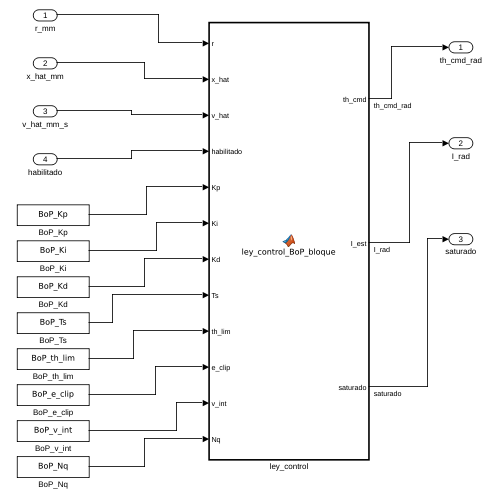
\includegraphics[width=0.85\columnwidth]{figuras/Controller_BoP_slx.png}
\caption{Modelo \texttt{Controller\_BoP.slx} (vista generada por Simulink): las cuatro entradas
de la interfaz, los ocho parámetros calibrables como bloques \texttt{Constant} y el bloque
\texttt{ley\_control}, que implementa \eqref{eq:ley}.}
\label{fig:controller}
\end{figure}

De la configuración de generación de código solo importan cuatro puntos para entender la
implementación. Se usó el destino \texttt{ert.tlc} de Embedded Coder con interfaz
\emph{Reusable function}, para que el estado viaje en una estructura y cada eje tenga la suya
\cite{mw_codegen}. Los datos son \texttt{double}. Los ocho parámetros del controlador son
\texttt{Simulink.Parameter} con clase de almacenamiento \texttt{ExportedGlobal}, así que quedan
como variables globales calibrables. Y el hardware se configuró como un procesador genérico de
\SI{32}{bits} \emph{little-endian}, con división entera que redondea hacia cero, que es lo que
permitió compilar el mismo código en la PC (SIL) y en la ESP32 (PIL). El Code Generation Advisor
dio \num{0} resultados Fail, \num{5} advertencias y \num{26} verificaciones aprobadas; las
advertencias se revisaron y justificaron una por una, sin usar correcciones automáticas.

Las cinco advertencias fueron: los objetivos de generación del Advisor no coincidían con los
fijados en el modelo (eficiencia y trazabilidad), lo que es informativo; el diagnóstico de nombres
duplicados de \emph{Data Store} no está en error, y el modelo no usa \emph{Data Stores}; el orden
de bytes y el redondeo de la división entera no estaban definidos, lo que se corrigió con la
configuración de hardware descrita arriba; el código admite números no finitos, que hacen falta
porque la función \texttt{sign} de MATLAB maneja \texttt{NaN}; y hay comparaciones de igualdad
entre valores en punto flotante, que son intencionales, porque \texttt{saturado} se define
como $\thc \ne u$.

\subsection{Inspección del código generado}

Antes de generar código se comprobó que el modelo reproduce el MIL: en cinco ensayos, incluido
uno con saturación, la diferencia entre el modelo y la ley usada en el MIL fue exactamente cero
en $\thc$, $I$ y \texttt{saturado}. Después se inspeccionó el código generado. La
Tabla~\ref{tab:codigo} resume la correspondencia.

\begin{table}[!t]
\caption{Correspondencia entre el modelo y el código generado (\texttt{Controller\_BoP.c} y
\texttt{.h}). Fuente: \texttt{etapaE/tabla\_modelo\_codigo.md}.}
\label{tab:codigo}
\centering
\footnotesize
\setlength{\tabcolsep}{3pt}
\begin{tabular}{@{}p{0.30\columnwidth}p{0.62\columnwidth}@{}}
\toprule
\textbf{Característica} & \textbf{Evidencia en el código} \\
\midrule
Interfaz & \texttt{Controller\_BoP\_step(M, r, x\_hat, v\_hat, hab, \&th, \&I, \&sat)}, tipos \texttt{real\_T} y \texttt{boolean\_T} \\
Estado interno & \texttt{DW\_Controller\_BoP\_T.I} y \texttt{.nq}, uno por instancia \\
Parámetros calibrables & \texttt{BoP\_Kp}, \texttt{BoP\_Ki}, \texttt{BoP\_Kd}, \texttt{BoP\_Ts}, \texttt{BoP\_th\_lim}, \texttt{BoP\_e\_clip}, \texttt{BoP\_v\_int}, \texttt{BoP\_Nq} como globales \\
Saturación & \texttt{fmin(fmax(u, -BoP\_th\_lim), BoP\_th\_lim)} \\
Integración condicional & \texttt{if (fabs(v\_hat) < BoP\_v\_int) nq++; else nq = 0;} \\
Anti-windup & El integrador no avanza si está saturado y $\operatorname{sign}(\varepsilon) = \operatorname{sign}(u)$ \\
Planta & Ausente: el código solo contiene la ley de control \\
\bottomrule
\end{tabular}
\end{table}

\begin{lstlisting}
a__1 = (BoP_Kp*eps_ + DW->I) + BoP_Kd*v_hat;
*th_cmd = fmin(fmax(a__1, -BoP_th_lim), BoP_th_lim);
\end{lstlisting}

El fragmento conserva el mismo orden de operaciones que el modelo. El código compilado con
\texttt{gcc} en la PC reprodujo el MIL con una diferencia máxima de \SI{4e-11}{\radian}, que
corresponde al redondeo de los CSV usados como referencia.

\subsection{Verificación Software-in-the-Loop}

El banco \texttt{BoP\_Test\_SIL.slx} tiene dos ramas en la misma simulación, Normal y SIL
\cite{mw_sil}. Comparten la referencia (cero y, a los \SI{4.5}{\second}, \SI{50}{\milli\metre} en
cada eje), la habilitación desde \SI{0.5}{\second}, la condición inicial de la bola en
$(80, -60)\,\si{\milli\metre}$, $\Ts$, la secuencia de ruido y el tiempo de \SI{9}{\second}. Cada
rama tiene su propia planta no lineal de dos ejes y sus dos instancias del controlador, porque
las acciones de control se calculan por separado. La Fig.~\ref{fig:sil} muestra la diferencia
$\Delta\theta_x = \theta_{x,\mathrm{SIL}} - \theta_{x,\mathrm{Normal}}$ y
$\Delta x = x_{\mathrm{SIL}} - x_{\mathrm{Normal}}$ junto con la trayectoria.

\begin{figure}[!t]
\centering
\begin{tikzpicture}
\begin{groupplot}[group style={group size=1 by 2, vertical sep=0.7cm}, estilo, height=3.2cm,
                  xmin=0, xmax=9]
\nextgroupplot[ylabel={Posición (\si{\milli\metre})}, xticklabels={}, legend pos=south east,
               legend columns=2]
  \addplot[cAzul] table[col sep=comma, x=t_s, y=Normal_x] {\G/F1_comparacion.csv};
  \addplot[cNaranja, dashed] table[col sep=comma, x=t_s, y=Normal_y] {\G/F1_comparacion.csv};
  \legend{$x$, $y$}
\nextgroupplot[ylabel={Diferencia}, xlabel={Tiempo (\si{\second})}, ymin=-1, ymax=1,
               legend pos=north east, legend columns=2]
  \addplot[cRojo] table[col sep=comma, x=t_s, y=dif_thx] {\G/F1_comparacion.csv};
  \addplot[cVerde, dashed] table[col sep=comma, x=t_s, y=dif_x] {\G/F1_comparacion.csv};
  \addplot[cNaranja, densely dotted, line width=1.1pt] table[col sep=comma, x=t_s, y=dif_thx] {\G/G5_comparacion.csv};
  \addplot[cAzul, dashdotted] table[col sep=comma, x=t_s, y=dif_x] {\G/G5_comparacion.csv};
  \legend{SIL $\Delta\theta_x$ (\si{\radian}), SIL $\Delta x$ (\si{\milli\metre}), PIL $\Delta\theta_x$, PIL $\Delta x$}
\end{groupplot}
\end{tikzpicture}
\caption{Bancos SIL y PIL. Arriba: trayectoria de la rama Normal. Abajo: diferencias
SIL $-$ Normal y PIL $-$ Normal (G5), idénticamente nulas en las \num{271} muestras.}
\label{fig:sil}
\end{figure}

En las \num{271} muestras y en las diez señales comparadas ($\thc$, $I$ y \texttt{saturado} de
cada eje, y $\xh$, $x$, $y$ de la planta) la diferencia máxima y el RMSE fueron cero, con igualdad
exacta (Tabla~\ref{tab:silpil}). La prueba satisface el criterio de equivalencia. SIL verifica
que el código generado, compilado en la PC, calcula lo mismo que el modelo dentro del lazo
cerrado. No verifica que funcione en la ESP32, ni con su compilador y su aritmética, ni con la
planta real. Además, este ensayo no lleva el controlador a la saturación; esa rama del código se
comprobó en la equivalencia previa y vuelve a probarse en PIL.

\section{Verificación Processor-in-the-Loop}

En PIL, el código del controlador se compila para el procesador objetivo y se ejecuta en él,
mientras la planta sigue simulada en la PC \cite{mw_pil}. El procesador es una ESP32 (ESP32-D0WD-V3,
placa de desarrollo de 38 pines), la misma que ejecuta el controlador en el prototipo.

El \emph{Simulink Support Package for Arduino Hardware} de R2026a programa la ESP32, pero no
habilita PIL para ella \cite{mw_arduino}: la clase de la placa declara
\texttt{IsPilSupported = 0}, y al registrar a mano una conexión PIL, la clase interna del paquete
falla porque espera datos que solo existen para las placas soportadas. Por eso se usó una
alternativa de ingeniería: un PIL propio con la misma arquitectura que el de Simulink. En la ESP32 corre exactamente el código C de la Etapa~E, el mismo
verificado en SIL (se comprueba que la copia sea idéntica byte a byte), compilado con la
cadena Xtensa del paquete, con dos instancias, una por eje. Un sketch hace solo de puente serie:
recibe $r$, $\xh$, $\vh$ y \texttt{habilitado} como \texttt{double} de \SI{8}{bytes}, llama a
\texttt{Controller\_BoP\_step}, y devuelve $\thc$, $I$, \texttt{saturado} y los ciclos de CPU de
la llamada. En la PC siguen la planta del banco SIL, la referencia, la rama Normal y la
comparación.

La Fig.~\ref{fig:pilarq} resume la arquitectura. El intercambio es por el puerto USB a
\SI{115200}{baudios}, un paso por mensaje, sin restricción de tiempo real.

\begin{figure}[!t]
\centering
\begin{tikzpicture}[font=\scriptsize, >=stealth,
  caja/.style={draw, rounded corners=1pt, align=center, minimum height=0.75cm, inner sep=2pt},
  grupo/.style={draw, dashed, rounded corners=2pt, inner sep=5pt}]
  \node[caja] (ref) {Referencia\\y habilitación};
  \node[caja, below=0.45cm of ref] (planta) {Planta de la rama PIL\\(2 ejes, Kalman)};
  \node[caja, below=0.45cm of planta] (normal) {Rama Normal\\(modelo y su planta)};
  \node[caja, right=0.4cm of normal] (cmp) {Comparación\\muestra a muestra};
  \node[grupo, fit=(ref)(planta)(normal)(cmp), label={[font=\scriptsize]above:PC (MATLAB)}] (pc) {};
  \node[caja, right=2.7cm of planta, minimum width=2.1cm] (step)
       {Puente serie\\$\downarrow$\\\texttt{Controller\_BoP\_step}\\(2 instancias)};
  \node[grupo, fit=(step), label={[font=\scriptsize]above:ESP32}] (esp) {};
  \draw[->] ([yshift=4pt]planta.east) -- node[above, font=\tiny, yshift=1pt]{$r, \xh, \vh$, hab.} ([yshift=4pt]step.west);
  \draw[<-] ([yshift=-4pt]planta.east) -- node[below, font=\tiny, yshift=-1pt]{$\thc, I$, sat.} ([yshift=-4pt]step.west);
  \draw[->] (ref) -- (planta);
  \draw[->] (normal) -- (cmp);
  \draw[->] (planta.south east) -- (cmp.north);
  \draw[->] (ref.west) -- ([xshift=-3mm]ref.west -| planta.west) |- (normal.west);
\end{tikzpicture}
\caption{Arquitectura del PIL propio. En la ESP32 corre solo el código generado; la planta, la
referencia, la rama Normal y la comparación siguen en la PC.}
\label{fig:pilarq}
\end{figure}

Se hicieron dos pruebas. En G4 se ejecutó el controlador solo, con las entradas del MIL de los
casos D1 y D2; el segundo tiene nueve cuadros saturados, así que ejercita la saturación y el
\emph{clamping} que el ensayo SIL no alcanzaba. En los dos casos $\thc$ e $I$ fueron idénticos y
ninguna bandera de saturación difirió. En G5 se repitió el banco de lazo cerrado de la
Sección~IV-C con la rama PIL. La Fig.~\ref{fig:pil} muestra las diferencias y la
Tabla~\ref{tab:silpil} resume las dos verificaciones.

\begin{figure}[!t]
\centering
\begin{tikzpicture}
\begin{axis}[estilo, height=3.2cm, xmin=0, xmax=9, ymin=-1, ymax=1,
             xlabel={Tiempo (\si{\second})}, ylabel={Diferencia}, legend pos=north east,
             legend columns=2]
  \addplot[cRojo] table[col sep=comma, x=t_s, y=dif_thx] {\G/G5_comparacion.csv};
  \addplot[cVerde, dashed] table[col sep=comma, x=t_s, y=dif_x] {\G/G5_comparacion.csv};
  \legend{$\Delta\theta_x$ (\si{\radian}), $\Delta x$ (\si{\milli\metre})}
\end{axis}
\end{tikzpicture}
\caption{Diferencias PIL $-$ Normal en el banco de lazo cerrado (G5).}
\label{fig:pil}
\end{figure}

\begin{table}[!t]
\caption{Resultados de las verificaciones SIL y PIL. LC: banco de lazo cerrado; G4: controlador
solo con las entradas del MIL ($\thc$, $I$ y \texttt{saturado}). Fuente:
\texttt{etapaF/resultados/F1\_metricas.csv}, \texttt{etapaG/resultados/G4\_resultados.csv} y
\texttt{G5\_metricas.csv}.}
\label{tab:silpil}
\centering
\footnotesize
\setlength{\tabcolsep}{3pt}
\begin{tabular}{@{}lccc@{}}
\toprule
 & \textbf{SIL (F1)} & \textbf{PIL (G4)} & \textbf{PIL (G5)} \\
\midrule
Ensayo & LC, 2 ejes & D1 y D2 & LC, 2 ejes \\
Muestras & 271 & 194 y 179 & 271 \\
Señales & 10 & 3 & 10 \\
$\max|\Delta|$ & 0 & 0 & 0 \\
RMSE & 0 & 0 & 0 \\
Igualdad exacta & 271/271 & Sí & 271/271 \\
Cuadros saturados & 0 & 9 (en D2) & 0 \\
\midrule
Resultado & PASS & PASS & PASS \\
\bottomrule
\end{tabular}
\end{table}

La igualdad exacta indica que el compilador Xtensa y la aritmética \texttt{double} de la ESP32,
que no tiene unidad de punto flotante de doble precisión y la emula por software, dan los mismos
resultados bit a bit que la PC para esta secuencia de operaciones. El tiempo de
\texttt{Controller\_BoP\_step} en la ESP32 fue de \SI{7.5}{\micro\second} de mediana y
\SI{31.3}{\micro\second} como máximo, el \SI{0.094}{\percent} de $\Ts$, así que el cálculo no
limita el periodo de muestreo.

PIL aporta, sobre SIL, la evidencia de que el código corre en el procesador objetivo, con su
compilador, y conserva el comportamiento. Aun así, un PASS en PIL no valida el controlador sobre
la planta real: la planta sigue siendo un modelo, no hay cámara ni servos, el intercambio por el
puerto serie no corre a \SI{30}{fps} en tiempo real, y el modelo usado para diseñar resultó, como
se vio en la Sección~II, bastante distinto del prototipo.

\section{Implementación experimental}

La implementación física no usó el código generado de \texttt{Controller\_BoP}. Por tiempo, el
equipo decidió probar el lazo con un firmware escrito a mano
(\texttt{firmware/bop\_controlador\_estable/}) que implementa la misma ley \eqref{eq:ley} con
las mismas ganancias. La función de la ley del primer firmware de prueba se comprobó,
compilada en la PC, contra la del MIL, con una diferencia máxima de \SI{6e-7}{\degree}, que
corresponde a la precisión simple del firmware. Sobre esa función se agregaron protecciones durante las pruebas: zona de tolerancia de
\SI{5}{\milli\metre}, tope del integrador en \SI{3}{\degree}, descarga del integrador lejos de la
referencia, límite de velocidad de \SI{6}{\degree} por cuadro, filtro de saltos de posición y un
\emph{trim} de nivel. Por eso los resultados de esta sección no son una validación del código
verificado en SIL y PIL, sino de la misma ley con esas protecciones.

\subsection{Arquitectura del lazo físico}

La cadena completa es: captura de la cámara a \SI{30}{fps} en la PC con Linux $\rightarrow$
homografía de píxeles a milímetros sobre el cuadrado de \SI{290}{\milli\metre} de las marcas del
plato $\rightarrow$ segmentación HSV de la bola con filtro de área y circularidad $\rightarrow$
corrección de paralaje $\rightarrow$ filtro de Kalman de velocidad constante $\rightarrow$ trama
binaria de \SI{20}{bytes} por el puerto serie a \SI{921600}{baudios} $\rightarrow$ controlador
en la ESP32 $\rightarrow$ saturación $\rightarrow$ conversión de inclinación a comando del servo
con la tabla medida $\rightarrow$ PWM de \SI{50}{\hertz} $\rightarrow$ servos. El
algoritmo de control se ejecuta en la ESP32; la PC solo mide y filtra. La ESP32 lleva el plato a
horizontal si la visión indica que no hay bola o si deja de recibir tramas durante
\SI{200}{\milli\second}, y en cada cuadro devuelve por el mismo puerto la inclinación aplicada,
que la PC guarda junto con la medición.

Las pruebas encontraron problemas de implementación que no estaban en el modelo y que se
corrigieron antes de medir: la ESP32 leía la trama byte a byte y trabajaba con datos unos
\SI{0.6}{\second} atrasados, los ejes de la cámara quedaron cruzados por el orden de los clics de
la calibración, y la primera tabla servo--plato tenía un desnivel en el neutro. Además, el
\texttt{loop()} de la ESP32 corre cada \SI{40}{\milli\second}, por lo que el controlador procesa
\num{25} de las \num{30} tramas por segundo.

Antes de energizar se comprobó: fuente de los servos separada de la ESP32, con interruptor a
mano y tierra común; primero se conecta la ESP32 y después la fuente; el firmware arranca
desarmado, con el plato horizontal, y solo actúa al presionar el botón BOOT; el comando del servo
se limita a $\pm\SI{40}{\degree}$; y el watchdog lleva el plato a horizontal si se pierden las
tramas. Durante las pruebas se agregaron al plato bordes más altos que impiden que la bola caiga.

\subsection{Resultados experimentales}

La Fig.~\ref{fig:exp} muestra los escalones de referencia de \SI{40}{\milli\metre} del ensayo
automático y una trayectoria circular de \SI{45}{\milli\metre} de radio y periodo de
\SI{4}{\second}, las dos con la pelota de ping pong y el controlador de la Sección~III. La
Tabla~\ref{tab:exp} resume las métricas de los escalones, calculadas desde el CSV con las
definiciones de la Sección~I, junto con las del MIL para escalones de \SI{50}{\milli\metre} (caso
D4). No es el mismo ensayo, porque en el prototipo no se corrió el ensayo de requisitos de
\SI{100}{\milli\metre}, pero sirve para comparar el orden de magnitud.

\begin{figure}[!t]
\centering
\begin{tikzpicture}
\begin{groupplot}[group style={group size=1 by 2, vertical sep=0.7cm}, estilo, height=3.2cm,
                  xmin=0, xmax=30]
\nextgroupplot[ylabel={$x$ (\si{\milli\metre})}, xticklabels={}, legend pos=north east,
               legend columns=2]
  \addplot[cAzul] table[col sep=comma, x=t_s, y=x_mm] {\G/exp_20261113_105834.csv};
  \addplot[cGris, densely dashed] table[col sep=comma, x=t_s, y=rx_mm] {\G/exp_20261113_105834.csv};
  \legend{Medida, Referencia}
\nextgroupplot[ylabel={$y$ (\si{\milli\metre})}, xlabel={Tiempo (\si{\second})}]
  \addplot[cNaranja] table[col sep=comma, x=t_s, y=y_mm] {\G/exp_20261113_105834.csv};
  \addplot[cGris, densely dashed] table[col sep=comma, x=t_s, y=ry_mm] {\G/exp_20261113_105834.csv};
\end{groupplot}
\end{tikzpicture}

\vspace{2mm}
\begin{tikzpicture}
\begin{axis}[estilo, width=0.5\columnwidth, height=0.5\columnwidth, axis equal image,
             xmin=-127, xmax=127, ymin=-127, ymax=127,
             xlabel={$x$ (\si{\milli\metre})}, ylabel={$y$ (\si{\milli\metre})}]
  \addplot[cAzul, line width=0.3pt, aligera=2,
           restrict expr to domain={\thisrow{modo}}{2:2}] table[col sep=comma, x=x_mm, y=y_mm] {\G/exp_20261113_105517.csv};
  \addplot[cRojo, dashed, domain=0:360, samples=73, line width=0.8pt] ({45*cos(x)}, {45*sin(x)});
\end{axis}
\end{tikzpicture}
\caption{Prueba funcional en el prototipo con el firmware de prueba. Arriba: escalones de
\SI{40}{\milli\metre} (\texttt{sesion\_20261113\_105834}). Abajo: trayectoria circular de
\SI{45}{\milli\metre} y \SI{4}{\second} durante \SI{157}{\second}, con el círculo pedido en rojo
(\texttt{sesion\_20261113\_105517}).}
\label{fig:exp}
\end{figure}

\begin{table}[!t]
\caption{Escalones en el prototipo (\texttt{sesion\_20261113\_105834}, tramos de
\SI{4.8}{\second}) y en MIL (D4). $\Delta$: cambio pedido desde la posición inicial; $e_f$: error
medio en el último segundo del tramo. Fuente: \texttt{informe/scripts/preparar\_datos.py} y
\texttt{etapaD/resultados/D1\_metricas.csv}.}
\label{tab:exp}
\centering
\footnotesize
\setlength{\tabcolsep}{3pt}
\begin{tabular}{@{}llrcrrr@{}}
\toprule
\textbf{Ensayo} & \textbf{Referencia} & $\Delta$ & $t_s$ & $M_p$ & $e_f$ & $\max|\thc|$ \\
 & (\si{\milli\metre}) & (\si{\milli\metre}) & (\si{\second}) & (\si{\percent}) & (\si{\milli\metre}) & (\si{\degree}) \\
\midrule
Prototipo, X & $0 \rightarrow 40$     & 40,7  & $> 4{,}7$ & 0 & 23,2 & 2,9 \\
Prototipo, X & $40 \rightarrow -40$   & -57,1 & $> 4{,}8$ & 0 & 27,8 & 1,9 \\
Prototipo, X & $-40 \rightarrow 0$    & 12,4  & $> 4{,}8$ & 0 & 9,3  & 1,3 \\
Prototipo, Y & $0 \rightarrow 40$     & 83,5  & $> 4{,}8$ & 0 & 80,5 & 2,0 \\
Prototipo, Y & $40 \rightarrow -40$   & 0,5   & $> 4{,}8$ & 0 & 38,6 & 1,6 \\
Prototipo, Y & $-40 \rightarrow 0$    & 76,7  & $> 4{,}8$ & 0 & 31,8 & 2,0 \\
\midrule
MIL D4, X & $0 \rightarrow 50$        & 51,3  & 4,00 & 14,1 & 1,5 & 2,1 \\
MIL D4, Y & $0 \rightarrow 50$        & 48,5  & 4,20 & 16,7 & 3,0 & 1,9 \\
\bottomrule
\end{tabular}
\end{table}

En el prototipo, ningún escalón se estableció dentro del tramo, así que $t_s$ solo tiene una
cota inferior, y el error al final fue de \SIrange{9}{80}{\milli\metre}, contra
\SIrange{1.5}{3.0}{\milli\metre} en el MIL. No hubo sobreimpulso: la bola se acerca lentamente y
se detiene antes de llegar. El eje Y fue el peor. En el escalón de 0 a \SI{40}{\milli\metre} la
bola estaba en \SI{-43}{\milli\metre} y prácticamente no se movió, aunque el plato llegó a pedir
\SI{2}{\degree}. Es el comportamiento que se espera de la zona muerta y la baja ganancia efectiva
identificadas en la Sección~II: con $\Kp = \SI{0.034}{\degree\per\milli\metre}$, un error de
\SI{30}{\milli\metre} pide apenas \SI{1}{\degree}, del orden de la zona muerta.

En el círculo, la órbita quedó centrada en $(6, -4)\,\si{\milli\metre}$, con un radio medio de
\SI{45}{\milli\metre} (percentiles 10 y 90 de \SI{16}{} y \SI{73}{\milli\metre}) y un error
mediano respecto de la referencia de \SI{30}{\milli\metre}. La bola estuvo a más de
\SI{115}{\milli\metre} del centro solo el \SI{0.2}{\percent} del tiempo, y se detectó en todos
los cuadros.

El 2026-11-18 se repitió el modo de centrado y apareció el mismo problema de forma más clara
(\texttt{sesion\_20261118\_092357}): la bola quedó \SI{55}{\second} quieta en
$(110, 58)\,\si{\milli\metre}$ con el plato pidiendo \SI{3.6}{\degree} y \SI{1.8}{\degree}, y el
integrador en cero, porque el firmware lo descargaba con la bola lejos de la referencia. Con eso
se corrigieron dos cosas: el \emph{trim} pasó a $\{1{,}5;\ 0{,}4\}\,\si{\degree}$, estimado como
la inclinación aplicada menos la zona muerta, y el integrador volvió a la regla de
\eqref{eq:ley}, que suma con la bola quieta en cualquier posición. En una simulación de un eje
con zona muerta, ese cambio dejó la bola a menos de \SI{13}{\milli\metre} del centro en los 30
casos probados, contra \SIrange{51}{57}{\milli\metre} en 3 casos con la regla anterior. Esta
última versión no se alcanzó a probar en el prototipo.

Con estos resultados, los requisitos R1 y R3 no se cumplen en la planta real. R4 tampoco se
cumplió siempre: en el log del 2026-11-18 la bola llegó al borde en $x \approx \SI{127}{\milli\metre}$,
y en las pruebas con la bola de PLA llegó a él decenas de veces. Fueron los bordes del plato los
que evitaron que cayera.

\section{Discusión}

\pendiente{Esta sección se termina con los datos de la Etapa~H. Lo que sigue es el esqueleto
con las diferencias ya medidas entre el modelo y la planta. Ordenarlas por peso cuando se tengan
los resultados finales y no corregirlas artificialmente.}

La diferencia principal entre el modelo y el prototipo está en la transmisión entre la orden de
inclinación y la bola. El modelo de diseño suponía $c = 5/7$ y un retardo de
\SI{75}{\milli\second}. La identificación dio una ganancia efectiva cercana a \num{0.2} para
movimientos pequeños y un retardo de \SIrange{0.27}{0.41}{\second}, con una zona muerta de
alrededor de \SI{1}{\degree}. Como el resultado fue el mismo con dos bolas muy distintas, el
origen está en el mecanismo: holgura de las rótulas y varillas, medida hasta \SI{2.4}{\degree}
en el eje Y, y respuesta del servo a cambios pequeños. El eje Y, cuyo servo es más duro, tiene
más holgura y más retardo, y es donde aparecieron casi todas las zonas en las que la bola se
quedaba trabada. La asimetría entre los ejes viene, entonces, del actuador.

Estas diferencias explican el comportamiento observado. Una ganancia de planta cuatro veces
menor queda cerca del margen de ganancia inferior de \SI{-12.6}{\deci\bel} del lazo
condicionalmente estable (Tabla~\ref{tab:controlador}), y un retardo cuatro veces mayor deja muy
poco margen de fase. Con un retardo total estimado de \SI{0.44}{\second} (cámara, datos de la
ESP32 y transmisión), el cálculo de márgenes del controlador original da un margen de fase de
unos \SI{12}{\degree} para $c_{\mathrm{ef}} = 0{,}2$, y un rediseño preliminar con ese modelo
($\Kp = \SI{0.00727}{\degree\per\milli\metre}$, $\Kd = \SI{0.0184}{\degree\per(\milli\metre\per\second)}$,
$\Ti = \SI{5}{\second}$) sube el margen a \SI{43}{\degree}. Con ese retardo, el requisito R1 de
\SI{3}{\second} no se puede cumplir con un controlador robusto: o se acepta un requisito menos
exigente o se reduce el retardo, con menos holgura mecánica y un \texttt{loop()} más rápido en la
ESP32.

\pendiente{Los márgenes del rediseño se calcularon fuera de MATLAB (Python, sesión del
2026-11-13). Antes de citarlos, repetir C1 y D1 en MATLAB con el modelo nominal identificado y
regenerar el código (E a G). Comparar en el prototipo el original y el rediseño con el mismo
ensayo: en las pruebas del 2026-11-13 el rediseño terminó más cerca en los escalones (error final
de \SIrange{1}{47}{\milli\metre}, contra \SIrange{9}{80}{\milli\metre}), pero siguió peor el
círculo (error mediano de \SIrange{45}{58}{\milli\metre}, contra \SI{30}{\milli\metre}).}

Otras diferencias identificadas: la latencia medida de la visión fue menor que la supuesta, el
ruido de posición fue unas diez veces menor que el \SI{1}{\milli\metre} del diseño (aunque, en
simulación, bajar el parámetro del Kalman a ese valor hacía oscilar el lazo, por lo que se
mantuvo en \SI{1}{\milli\metre}), la relación servo--plato fue asimétrica y más empinada que la calculada, y
el término centrífugo limita la validez del modelo lineal cuando el plato se mueve rápido.

\pendiente{Diferencias de la implementación física (cuantización, efecto del \texttt{loop()} de
\SI{40}{\milli\second}, la zona de tolerancia de \SI{5}{\milli\metre} y su efecto sobre R3,
perturbaciones por choques con el borde) cuando se tengan los datos de H.}

\section{Conclusiones}

El modelo físico mostró que, por eje, la planta es un doble integrador que no es estable en lazo
abierto. Por eso no aplicaban ni las reglas SIMC ni un PI, y la identificación tuvo que hacerse en
lazo cerrado. El modelo lineal es válido hasta unos \SI{3}{\degree} con cambios lentos de
inclinación, pero solo hasta \SI{0.5}{\degree} con cambios rápidos, por el término centrífugo.

Con el modelo de diseño, el controlador PD con integración condicional cumplió los requisitos en
MIL ($t_s = \SI{1.30}{\second}$, $M_p = \SI{4.4}{\percent}$, $e_{ss} = \SI{0.18}{\milli\metre}$),
mientras que el PID clásico llegó a \SI{38.8}{\percent} de sobreimpulso. La saturación de
\SI{10}{\degree} que impone el mecanismo no alcanza para frenar un empujón de
\SI{420}{\milli\metre\per\second} antes del borde.

El código generado con Embedded Coder fue equivalente al modelo en SIL y en PIL sobre la ESP32,
con igualdad exacta en todas las muestras y \SI{31.3}{\micro\second} de cálculo como máximo. Para
el PIL hubo que construir una ruta propia, porque el paquete de soporte de Arduino no lo habilita
para la ESP32. Estos resultados verifican el código, no el desempeño sobre la planta.

La identificación sobre el prototipo dio una ganancia efectiva de \numrange{0.12}{0.28}, un
retardo de unos \SI{0.3}{\second} y una zona muerta de alrededor de \SI{1}{\degree}, atribuibles
al mecanismo. El modelo de diseño no representa bien el prototipo, y eso explica que en la planta
real no se cumplieran R1 ni R3: los escalones no se establecieron en \SI{4.8}{\second} y
terminaron a entre \SI{9}{} y \SI{80}{\milli\metre} de la referencia, aunque sin sobreimpulso. El
seguimiento de un círculo de \SI{45}{\milli\metre} sí funcionó, con un error mediano de
\SI{30}{\milli\metre}.

Las limitaciones principales del trabajo son tres. La implementación física usó un firmware
escrito a mano con la misma ley, y no el código generado. El rediseño con el modelo identificado
solo se evaluó en el prototipo. Y la última versión del firmware, con el integrador corregido y el
nivel reajustado, no se alcanzó a probar. Para mejorar el desempeño hace falta, antes que otro
controlador, reducir la holgura y el retardo del mecanismo, sobre todo en el eje Y.


\balance
\bibliographystyle{IEEEtran}
\bibliography{referencias}

\end{document}
